%!TEX root = ../masters_thesis.tex

\chapter{Development} % (fold)
\label{cha:development}

The aim of this thesis is to create a Historical Geographic Information System to visualize and edit the evolution of countries in time and space. This is a complicated task, because both the reality and the human that should be able to use the system are complex. The task is to create an interface that a human can easily understand and use. For complex applications in which the interface matters, the methodologies of \emph{Human Centered Design} are promising to achieve a good solution.

The development process is iterative divided in several phases. In each phase, the fidelty towards the final solution is increased. A phase starts with an initial set of requirements about the problem. In multiple iterations, an interface is developed that solves the problem. Each iteration has four steps: The requirements for the system are analyzed in the \emph{planning} step. Afterwards, they translated into an abstract \emph{design} which is realized in a specific \emph{implementation} of the interface. Finally, this interface is tested with humans to find out how well it works. Based on the results of this \emph{testing} step, the requirements are updated and the next iteration starts. This is repeated until a version of the interface is created that sufficiently solves the problem. Then the fidelity is increased, starting the next development phase.


% graphic: iterations
% idea -> interviews -> paper prototype -> mockup prototype -> final interface -> application -> extension
The five phases in this thesis were:
\begin{compactenum}
  \item \textbf{Idea}: The initial idea how to edit and visualize the history of countries.
  \item \textbf{Paper Prototype}: The concept of the interface realized and tested on paper.
  \item \textbf{Mockup Prototype}: The concrete workflow developed in a slide-based presentation.
  \item \textbf{Web-Based Prototype}: The final version developed in a Web application.
  \item \textbf{Extensions}: Design approaches how to fit the uncertain nature of history.
\end{compactenum}

\begin{figure}[H]
  \centering
  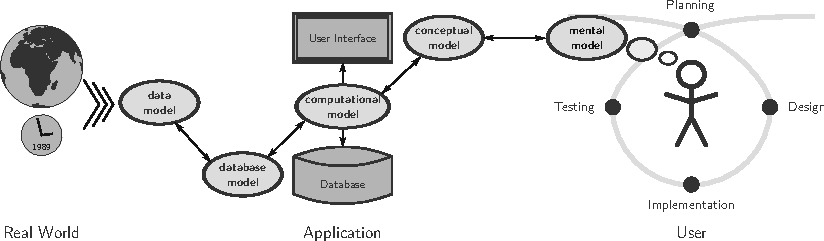
\includegraphics[width=0.8\textwidth]{graphics/development/hcd_models}
  \caption{Human Centered Design and relevant models for the system}
  \label{fig:hcd_models}
\end{figure}

The \emph{data model} is an abstraction and simplification of the real world. The \emph{Hivent Model} created in this thesis is explained in the first section \ref{sec:hivent_model} of this chapter. In iteractive computer systems, the \emph{mental model} is the representation in the mind of the human about how the interface he or she is interacting with should work. On the other hand, the \emph{conceptual model} describes the way the interface actually works. The goal of Human Centered Design is to match the conceptual model to the mental model. Section \ref{sec:histoglobe_interface} outlines the gradual interface design process to reach this goal. In the application, the implemented \emph{database model} has to match the abstract data model. The task for the \emph{computational model} is to translate between the database model and the conceptual model. The working of the HistoGlobe application, including the computational model, is introduced in the last section \ref{sec:histoglobe_application} of this chapter.

% ==============================================================================
\section{Hivent Model} % (fold)
\label{sec:hivent_model}

This section introduces the data model that represents countries and their evolution in time and space. In section \ref{sec:spatio_temporal_data_models}, different spatio-temporal data models were introduced to solve this problem. The \emph{Snapshot Model} is unsuitable for the problem space. \emph{Simple Time-Stamping} is helpful to link countries to their history, it does not explicitly model historical changes, which is desireable. For that purpose, the idea of the \emph{Event-Based Spatio-Temporal Data Model} was developed, but since it only works for raster data, it is also not suitable for this thesis. This problem is solved in the \emph{History Graph Model}. Additionally, the introduced temporal changes allow to represent historical changes and their influences on geographic entities directly in the model. Finally, the \emph{Three-Domain Model} introduces a helpful concept to separate the spatial, temporal and thematic dimension of a spatio-temporal entity.

The \emph{Hivent Model} is constructed from components of some of these models: An Event-Based Spatio-Temporal Data Model supporting vector data. It is organized according to the Three-Domain Model, uses Simple Time-Stamping to define the lifetime of a spatial entity, and to visualize it on a History Graph. In the first section of this section, the main elements of the Hivent model are introduced. Afterwards, the preconditions are defined. Finally, the Historical Geographic Operations that describe changes of countries in time and space are explained.

% ------------------------------------------------------------------------------
\subsection{Elements} % (fold)
\label{sub:elements}

The main elements of the the model are \emph{Hivent}s, representing an historically significant happening and \emph{Area}s, an abstract entity on a map with a name and a territory. An \emph{Historical Change} is part of one Hivent and manipulates the history of one or more Areas.

% - - - - - - - - - - - - - - - - - - - - - - - - - - - - - - - - - - - - - - -
\paragraph{Hivents} % (fold)
\label{par:hivent}

are the main organizing elements of the data model. The word is an acronym for \emph{\textbf{Hi}}storical e\emph{\textbf{vent}}. It represents a significant happening in history, e.g. a treaty, bill or declaration. The focus in this work is on events that influence the geopolitical situation on Earth. An Hivent happens at one particular point in time and space and introduces historical changes to countries.

% paragraph hivent (end)

% - - - - - - - - - - - - - - - - - - - - - - - - - - - - - - - - - - - - - - -
\paragraph{Areas} % (fold)
\label{par:area}

represent one identical current or historical country with a \emph{name} and a \emph{territory} on the map. The name of the Area consists of a common \emph{short name}, e.g. ``Germany'' and a \emph{formal name}, e.g. ``Federal Republic of Germany''. The \emph{territory} of the Area is described by a polypolygon, a set of weakly simple polygons to support enclaves and exclaves. The polylines of the polygons consist of an ordered set of points that represent the country border.

% paragraph area (end)

% ------------------------------------------------------------------------------
\paragraph{Historical Changes} % (fold)
\label{par:historical_changes}

influence the development of an Area over time. Throughout the lifetime of an Area, it is created at some point $t_s$, then its territory and short name can change multiple times $t_i: t_s < t_i$ and at some point $t_e: t_s < t_i < t_e$ it ceases. Since all changes in this model are sudden, there are only two possible states an Area can be in: It is \emph{active}, if at the current time point it is historically existing and it is \emph{inactive} if it does not. Each area is uniquely identified by its formal name. That means, the short name can change, but as soon as the formal name of an area changes (e.g. ``German Empire'' to ``Federal Republic of Germany''), it is considered a ``new'' Area.

\begin{figure}[H]
  \vspace{1em}
  \centering
  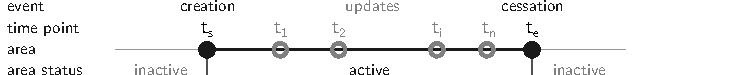
\includegraphics[width=0.9\textwidth]{graphics/development/area_states}
  \caption{Three event types that change Areas, resulting in two different area states}
  \label{fig:area_states}
\end{figure}

Each Historical Change belongs to exactly one Hivent, inheriting its time point at which the change happens.  The change is described by a Historical Geographic Operation introduced in section \ref{sub:historical_geographic_operations}.

% paragraph historical_changes (end)

% subsection section area (end)

% ------------------------------------------------------------------------------
\subsection{Preconditions} % (fold)
\label{sub:preconditions}

\begin{quoteit}
In the beginning God created the heavens and the Earth \\
Now the Earth was formless and empty [...] \\
And God said, “Let there be light” --- and there was light.
\end{quoteit}
\hfill -- Genesis 1:1, The First Book of Moses, Old Testament

The spatio-temporal system has to be initialized at some point. It is based on a set of trivial axioms stated in this section. Each Area in the system is located directly on the surface of the Earth. While the surface is curved, as explained in sections \ref{sub:model_of_geographical_space} and \ref{sub:presentation_of_geographic_space}, it can be projected on a two-dimensional map.

\vspace{-1.0em}
\newtheorem{invariant_surface}[assicounter]{Axiom}
\begin{invariant_surface}
\label{axm:invariant_surface}
  The Earth's surface has an invariant area size, i.e. it does not change over time.
\end{invariant_surface}

This axiom sets the spatial foundation of the system: a constant dimension of the map. The basis of the temporal part of the system is introduced in the next three axioms:

\vspace{-1.0em}
\newtheorem{initial_configuration}[assicounter]{Axiom}
\begin{initial_configuration}
\label{axm:initial_configuration}
  The spatio-temporal system has an initial state at time point $t_0$. At this initial state, there exists exactly one Area, denoted by $\Omega$ and referred to as the \emph{universe} Area. It has no name and its territory covers the whole surface of the Earth.
\end{initial_configuration}

\vspace{-1.5em}
\newtheorem{historical_change}[assicounter]{Axiom}
\begin{historical_change}
\label{axm:historical_change}
  At each time point $t_i \geq t_0$ an Historical Change can be introduced.
\end{historical_change}

\vspace{-1.5em}
\newtheorem{unique_coverage}[assicounter]{Axiom}
\begin{unique_coverage}
\label{axm:unique_coverage}
  At each time point $t_i \geq t_0$ each point on the surface of the Earth is covered by exactly one territory of exactly one Area.
\end{unique_coverage}

As it has been defined in section \ref{par:historical_changes}, an Historical Change can create, manipulate and cease Areas on the Earth's surface. According to axoim \ref{axm:unique_coverage}, each change introduced in the system must maintain the spatial integrity on the map. That means, as soon as an Area is created in one territory on the map, the territory that was there before has to cease. Vice versa, if an Area ceases from the map, it has to be replaced with at least one new Area and these new Areas combined have to occupy exactly this same territory.

The first Historical Changes introduced in the system at time point $t_0$ are the creation of all bodies of water, including the oceans and lakes. They are created as Areas with their name and territory which is cut out of $\Omega$. That means, at $t_0$, the map of the world is divided into a set of Areas representing water and $\Omega$, representing land. Land can at any point in time be either \emph{claimed}, i.e. it is currently occupied by the territory of exactly one active Area, or on a contrary be \emph{unclaimed}, i.e. belonging to $\Omega$. It is a subtractive data model, because each Area that is created new will be cut out of $\Omega$.

The borders of a country are either \emph{interior}, i.e. bordering another country, or a \emph{coastline}, bordering a body of water. This assumption is a concious simplification of the reality: It assumes the territory of a country stops at the coastline. Juristically, this is not true, because in line with \cite{UNSeaBorders}, the territory extends in a range of 3 to 12 miles (5 to 20 kilometers) into international waters. This model disregards the sea territory of a political entity to keep the model simple.

In the real world, The name of a country changes according to sudden events, e.g. a declaration or a governmental bill. The territory can change either because of a geographical processes, e.g. the Sea Level Rise influencing the change of the coastline, or according to a historical event, e.g. a treaty.

\vspace{-1.0em}
\newtheorem{constant_coastlines}[assicounter]{Assumption}
\begin{constant_coastlines}
\label{axm:constant_coastlines}
  The spatial configuration of the Earth's surface, i.e. land, water and the coastlines, has not changed over time.
\end{constant_coastlines}

While this assumption is obviously wrong, it helps to keep the problem space clear and the Hivent Model simple: it focuses only on discrete historical changes and not on long-term processes. However, it is open to future extensions to account also for geographic changes and international sea borders. In this data model, the temporal behavior of an Area can therefore be described as a \emph{static object that changes according to sudden events}.

% base: Newtons concept of absolute space?
% TODO: topological rule?
% each border has exactly two neighboring Areas
% each Area has at least one neighboring Area

% subsection preconditions (end)

% ------------------------------------------------------------------------------
\subsection{Historical Geographic Operations} % (fold)
\label{sub:historical_geographic_operations}

Respecting the preconditions, there are five different types of changes that can occur to a set of Areas. They can be expressed with five spatio-temporal operations which are called \emph{Historical Geographic Operations} (HG Operations). Four of them change the identity of a set of Areas and therefore establish historical predecessor-successor-relationships. That means, if one old Area is replaced by one new Area, the old Area is the historical predecessor of the new Area and vice versa the new Area is the successor of the old Area.
% Historical relationships are only noted in one direction (predecessor), but are always valid also in the other direction (successor).

\begin{description}
  \item[UNI -- Unification]
  A set of old Areas unifies to ome new Area. The old Areas cease, becoming the historical predecessors of the new Area. This new Area receives a new name and its territory is the union of the territories of the old Areas. \\
  \begin{footnotesize}
    In 1922, the Russian SFSR, the Transcaucasian SFSR, the Ukrainian SSR and the Byelorussian SSR unified and formed the Union of Soviet Socialist Republics (USSR).
  \end{footnotesize}
  \item[INC -- Incorporation]
  One or more old Areas are incorporated into another Area that stays active. Its territory is enlarged by the union of the territories of the old Areas. The old Areas are historical predecessors of the new Area. \\
  \begin{footnotesize}
    In 1990, the territory of the German Democratic Republic (East Germany) became part of the Federal Republic of Germany (West Germany). Although this event is known as the \emph{German Reunification}, it is historically an incorporation of East Germany into West Germany \cite{incorporationEastWestGermany}.
  \end{footnotesize}
  \item[SEP -- Separation]
  As the inverse of unification, one old Area is preceded by multiple new Areas. Each new Area gets a new name, receives a part of the territory of the old Area, and the old Area as its only historical predecessor. \\
  \begin{footnotesize}
    In 1993, the Czech and Slovak Federal Republic, commonly known as Czechoslovakia, dissolved into present-day Czech Republic and Solvak Republic, creating two new countries.
  \end{footnotesize}
  \item[SEC -- Secession]
  As the inverse of incorporation, one or more new areas are ceded from a previously exising area that stays active. Each new Area gets a new name, receives the previously existing Area as the only historical predecessor and a part of its territory. \\
  \begin{footnotesize}
    In 2008, the Republic of Kosovo declared independence from Serbia and has since then partially received international recognition. Unlike in the case of separation, Serbia stays as country, keeping its name, but ceding a part of its territory to Kosovo.
  \end{footnotesize}
  \item[NCH -- Name Change]
  An Area changes its short name but preserves its identity. \\
  \begin{footnotesize}
    A recent change happened on 5. May 2016: The cabinet of Czech Republic approved that the country will now offically be called ``Czechia''. The formal name stays ``Czech Republic''.
  \end{footnotesize}
\end{description}

% - - - - - - - - - - - - - - - - - - - - - - - - - - - - - - - - - - - - - - -
\begin{table}[H]
\begin{center}
\begin{tabular}{m{0.75cm} m{2.5cm} m{2.5cm} m{2.0cm} m{2.5cm}}
  \toprule
  & operation
  & \multicolumn{1}{c}{visualization}
  & \multicolumn{1}{c}{\pbox{2.5cm}{historical\\relationship}}
  & \multicolumn{1}{c}{territory} \\

  \midrule
  \texttt{UNI} & Unification & \raisebox{-0.25\height}
  {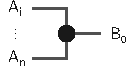
\includegraphics{graphics/development/operations/UNI}} &
  $ A_i \leftrightarrow_H B $ &
  $ B^T = \cup_{i=1}^{n} A_i $ \\

  \midrule
  \texttt{INC} & Incorporation & \raisebox{-0.25\height}
  {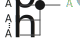
\includegraphics{graphics/development/operations/INC}} &
  $ A_i \leftrightarrow_H A_0 $ &
  $ A_0^T = \cup_{i=1}^{n} A_i $ \\

  \midrule
  \texttt{SEP} & Separation & \raisebox{-0.25\height}
  {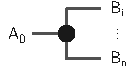
\includegraphics{graphics/development/operations/SEP}} &
  $ A \leftrightarrow_H B_i $ &
  $ B_i^T \cap A^T = B_i^T $ \\

  \midrule
  \texttt{SEC} & Secession & \raisebox{-0.25\height}
  {
\includegraphics{graphics/development/operations/SEC}} &
  $ A_i \leftrightarrow_H A_0 $ &
  $ B_i^T \cap A^T = B_i^T $ \\

  \midrule
  \texttt{NCH} & Name Change & \raisebox{-0.25\height}
  {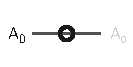
\includegraphics{graphics/development/operations/NCH}} &
  $ \emptyset $ &
  $ \emptyset $ \\

  \bottomrule
\end{tabular}
\caption{Overview about the five HG Operations}
\label{tab:historical_geographic_operations}
\end{center}
\end{table}


% subsection historical_geographic_operations (end)

% section hivent_model (end)

% ==============================================================================
\section{HistoGlobe Interface} % (fold)
\label{sec:histoglobe_interface}

understand the visualization
be able to edit the data

- the final version of the conceptual model for the user: Hivent
- the gradual process of interface design (PP -> MP -> HG)

% ------------------------------------------------------------------------------
\subsection{Edit Operations} % (fold)
\label{sub:Edit_operations}

CRE
UNI
SEP
BCH
NCH
CES

% subsection Edit_operations (end)

% ------------------------------------------------------------------------------
\subsection{Edit Mode} % (fold)
\label{sub:edit_mode}


geometries must be edited

% subsection edit_mode (end)

% ------------------------------------------------------------------------------
\subsection{HistoGraph} % (fold)
\label{sub:histograph}

% subsection histograph (end)

% ------------------------------------------------------------------------------
\subsection{Design Iterations} % (fold)
\label{sub:design_iterations}

% - - - - - - - - - - - - - - - - - - - - - - - - - - - - - - - - - - - - - - -
\paragraph{Paper Prototype} % (fold)
\label{par:paper_prototype}

description of process
image of two prototypes

% paragraph paper_prototype (end)

% - - - - - - - - - - - - - - - - - - - - - - - - - - - - - - - - - - - - - - -
\paragraph{Mockup Prototype} % (fold)
\label{par:mockup_prototype}

description of process
screenshot of two steps in between and of final version

% paragraph mockup_prototype (end)

% - - - - - - - - - - - - - - - - - - - - - - - - - - - - - - - - - - - - - - -
\paragraph{HistoGlobe Interface} % (fold)
\label{par:histoglobe_interface}

screenshot
explanation of all final UI Elements

% paragraph histoglobe_interface (end)

% subsection design_iterations (end)

% section histoglobe_interface (end)


% ==============================================================================
\section{HistoGlobe Application} % (fold)
\label{sec:histoglobe_application}

- the final version of the application behind the interface built on top of the data model

distributed Web-based system
classic approach: UI <-> Client (main program) <-> Server (middleware) <-> DB

% ------------------------------------------------------------------------------
\subsection{System Architecture} % (fold)
\label{sub:system_architecture}


The system developed in this thesis is Web-based. That means, there is a \emph{client}, a Web browser, and a remote Web \emph{server} with a database and a middleware. The Web browser hosts the applications user interface. If the user interacts with a tool the client sends a request to the Web server for new data. The middleware checks the request and queries the necessary data from the database. The data will be transformed and sendt back to the client. On the map and the timeline the new information will be shown.

This clear separation between the data (\emph{model}), the user interface (\emph{view}) and the middleware (\emph{controller}) follows directly from the \emph{model-view-controller pattern}: One part can be changed without interfering the other parts, e.g. if the 2D map is replaced by a 3D globe, only the view changes, but the middleware and the database can stay untouched. Likewise, the implementation of a new database technology has no consequences to the view.

graphic of basic system:
UI
Client-side mechanism
Server-side mechanism
Database

programming languages / Framworks
Client                    HTML
          Less ->         CSS
          CoffeeScript -> JavaScript
Server    Django ->       Python
                          PostgreSQL
                          + PostGIS

% subsection system_architecture (end)

% ------------------------------------------------------------------------------
\subsection{Database Model} % (fold)
\label{sub:database_model}

database model

\begin{compactenum}
  \item The \emph{name} of the Hivent.
  \item A textual \emph{description} of the topic of the Hivent.
  \item The point in time, identified by the Hivent \emph{date}.
  \item The Hivent \emph{location}.
  \item The \emph{historical changes} resulting from the Hivent.
\end{compactenum}


           Hivent
             m
       HistoricalChange
             m
  --------AreaChange------
  |          |           |
  |     ----Area----     |
  m     m          m     m
AreaTerritory      AreaName

no transaction time, only valid / event time
only world time is regarded, not database time.

view

get\_all
save\_operation

% subsection database_model (end)


% ------------------------------------------------------------------------------
\subsection{Computational Model} % (fold)
\label{sub:computational_model}

Class diagram

HistoGlobe

SpatialDisplay -> Map

TimeController  <-> Timeline
                <-> NowMarker

HiventController                AreaController <->  AreasOnMap
HiventHandle                    AreaHandle
Hivent
HistoricalChange    AreaChange  Area
                                AreaName            AreaNameLayerOnMap
                                AreaTerritory       AreaTerritoryLayerOnMap

DatabaseInterface

EditMode -> EditOperation -> EditOperationStep
NewTerritoryTool* NewNameTool NewHiventBox
WorkflowWindow

HistoGraph

LabelManager*

important little utils
  Button, ButtonArea
  NumberInput, TextInput, TextInputArea
  Title
  Watermark
  DoublyLinkedList
  WithinTree
  Geometry -> Polypolygon -> Polygon -> Polyline -> Point

% - - - - - - - - - - - - - - - - - - - - - - - - - - - - - - - - - - - - - - -
translation

Edit Operations   CRE   UNI   SEP   TCH   NCH   DES

HG Operations     UNI   INC   SEP   SEC   NCH

% - - - - - - - - - - - - - - - - - - - - - - - - - - - - - - - - - - - - - - -
\paragraph{Functional description} % (fold)
\label{par:functional_description}

Each HG Operation can be described by a mathematical function. The following symbols are used in the equations:

\begin{addmargin}[1em]{0em}
\begin{tabbing}
  symbolxx \= description1xx \= description2 \kill
  $A$ \> set of old Areas that were active before the Historical Change \\
  $B$ \> set of new Areas that are created in the Historical Change \\
  $n:$ \> $n \in \mathbb{N}, n>0$ \> total number of old respectively new Areas \\
  $i:$ \> $i \in [\textbf{1} .. n]$ \> iterator for the current old respectively new Area \\
  $A_0/B_0$ \>    the first old respectively new Area ($i \geq 1 \Rightarrow$ not $A_i/B_i$~!) \\
  $A_i/B_i$ \>    the current old respectively new Area ($i \geq 1 \Rightarrow$ not $A_0/B_0$~!) \\
  $A_i^T/B_i^T$ \>the new territory of the current Area (a polypolygon) \\
  $A_i^N/B_i^N$ \>the new name of the current Area (short and formal name) \\
\end{tabbing}
\end{addmargin}

\vspace{-2.5em}
\begin{align*}
  (B_0)                       &= UNI([A_1 .. A_i .. A_n], B_0^N) \\
  (A_0)                       &= INC(A_0, [A_1 .. A_i .. A_n]) \\
  ([B_1 .. B_i .. B_n])       &= SEP(A_0, [[B_1^T, B_1^N] .. [B_i^T, B_i^N] .. [B_n^T, B_n^N]]) \\
  (A_0, [B_1 .. B_i .. B_n])  &= SEC(A_0, A_0^T, [[B_1^T, B_1^N] .. [B_i^T, B_i^N] .. [B_n^T, B_n^N]]) \\
  (A_0)                       &= NCH(A_0, A_0^N)
\end{align*}

% paragraph functional_description (end)

% - - - - - - - - - - - - - - - - - - - - - - - - - - - - - - - - - - - - - - -
\paragraph{Pseudocode description} % (fold)
\label{par:pseudocode_description}

of the HG operations in an object-oriented manner. The existance of a class \texttt{Area} is assumed. Each \texttt{Area} object has the following member variables: a \texttt{name}, a \texttt{territory} and a list of historical \texttt{predecessors} and \texttt{successors}. Single capital letter variables (\texttt{A}/\texttt{B}) denote arrays of \texttt{Area} objects. Variables with a capital letter followed by a number or lowercase letter (e.g. \texttt{B0}) are single \texttt{Area} objects.

\begin{minipage}[t]{0.47\textwidth}
\begin{lstlisting}[language=pseudocode,
  caption=Unification]
FUNCTION UNI(A, B0_name)
  # create new territory
  B0_territory = NEW Geometry # empty
  FOREACH Ai IN A
    B0_territory.union(Ai.territory)
  # create new area
  B0 = NEW Area(B0_name, B0_territory)
  # establish historical relationships
  FOREACH Ai IN A
    Ai.successors.add(B0)
    B0.predecessors.add(A1)
  # return new area
  RETURN B0
\end{lstlisting}
\end{minipage}    % N.B. the % is very important
\hspace{3.0em}    % N.B. this must go in this line, no blank lines !!!
\begin{minipage}[t]{0.47\textwidth}
\begin{lstlisting}[language=pseudocode,
  caption=Incorporation]
FUNCTION INC(A0, A)
  # update old area with new territory
  temp_terr = NEW Geometry # empty
  FOREACH Ai IN A
    temp_terr.union(Ai.territory)
  A0.territory = temp_terr
  # establish historical relationships
  FOREACH Ai IN A
    Ai.successor.add(A0)
    A0.predecessor.add(A1)
  # return new area
  RETURN A0
\end{lstlisting}
\end{minipage}

\begin{minipage}[t]{0.47\textwidth}
\begin{lstlisting}[language=pseudocode,
  caption=Separation]
FUNCTION SEP(A0, B_data)
  # create each new Area
  B = []
  FOREACH Bi_data in B_data
    B.add(NEW Area(
      Bi_data.name, Bi_data.territory)
    )
  # establish historical relationships
  FOREACH Bi IN B
    A0.successors.add(Bi)
    Bi.predecessors.add(A0)
  # return new areas
  RETURN B

\end{lstlisting}
\end{minipage}    % N.B. the % is very important
\hspace{3.5em}    % N.B. this must go in this line, no blank lines !!!
\begin{minipage}[t]{0.47\textwidth}
\begin{lstlisting}[language=pseudocode,
  caption=Secession]
FUNCTION SEC(A0, A_territory, B_data)
  # update old area with new territory
  A0.territory = A_territory
  # create each new Area
  B = []
  FOREACH Bi_data in B_data
    B.add(NEW Area(
      Bi_data.name, Bi_data.territory)
    )
  # establish historical relationships
  FOREACH Bi IN B
    A0.successors.add(Bi)
    Bi.predecessors.add(A0)
  # return old and new areas
  RETURN [A0, B]

\end{lstlisting}
\end{minipage}

\vspace{-1.5em}
\begin{minipage}[t]{0.47\textwidth}
\begin{lstlisting}[language=pseudocode,
  caption=Name Change]
FUNCTION NCH(A0, A_name)
  # update old area with new name
  A0.name = A_name
  # return updated area
  RETURN A0

\end{lstlisting}
\end{minipage}

% paragraph pseudocode_description (end)


\paragraph{Execute Historical Change} % (fold)
\label{par:execute_historical_change}

execute function for all operations the same

% - - - - - - - - - - - - - - - - - - - - - - - - - - - - - - - - - - - - - - -
\begin{lstlisting}[language=pseudocode,
  caption=class HGOperation]
## member variables
old_areas = []          # Area
new_areas = []          # Area
update_name = {
  area :          null  # Area
  old_name :      null  # AreaName
  new_name :      null  # AreaName
}
update_territory = {
  area :          null  # Area
  old_territory : null  # AreaTerritory
  new_territory : null  # AreaTerritory
}

## main function
FUNCTION execute(direction)

  # hide old areas
  FOREACH old_area IN old_areas
    IF direction IS 1 # forward change
      old_area.hide()
    ELSE              # backward change
      old_area.show()

  # show new areas
  FOREACH new_area IN new_areas
    IF direction IS 1 # forward change
      new_area.show()
    ELSE              # backward change
      new_area.hide()

  # check if the area name is updated
  IF update_name.area
    IF direction IS 1 # forward change
      update_name.area.name = new_name
    ELSE              # backward change
      update_name.area.name = old_name
    update_name.area.update()

  # check if the area territory is updated
  IF update_territory.area
    IF direction IS 1 # forward change
      update_territory.area.territory = new_territory
    ELSE              # backward change
      update_territory.area.territory = old_territory

\end{lstlisting}

% paragraph execute_historical_change (end)

% subsection computational_model (end)

% section histoglobe_application (end)

% chapter development (end)

% ==============================================================================

\vspace{2em}
transition to next chapter